\documentclass[aps,pra,twocolumn,superscriptaddress,longbibliography,floatfix]{revtex4-2}
\usepackage{graphicx}
\usepackage{amsmath,amssymb}
\usepackage{bm}
\usepackage[colorlinks=true,allcolors=blue]{hyperref}
\newcommand{\um}{\,\mu\mathrm{m}}
\newcommand{\us}{\,\mu\mathrm{s}}
\newcommand{\MHz}{\,\mathrm{MHz}}
\newcommand{\todo}[1]{\textbf{[#1]}}

\begin{document}

\title{Blackbody-induced Rydberg \textit{P}-state contaminants in parallel gate layers:\\ error per contaminant, inter-gate delay and a density floor}

\author{\todo{CONFIRM?: author list}}
\affiliation{\todo{CONFIRM?: affiliation}}

\date{\today}

\begin{abstract}
In neutral-atom processors that execute many controlled-$Z$ (CZ) gates in parallel, blackbody radiation transfers a small fraction of the Rydberg-excited atoms to neighbouring $P$ states. These contaminants survive for about $100\us$ at room temperature and perturb gates at other sites through resonant dipole exchange. The effect has been observed and removed experimentally by increasing the time or the distance between gates [Bluvstein \textit{et al.}, arXiv:2506.20661]. We give a quantitative account of it with no fitted parameter. For the published $^{87}$Rb $53S_{1/2}$ time-optimal gate at $\Omega/2\pi=4.6\MHz$, a contaminant is created with probability $2.5\times10^{-4}$ per atom per gate at $300$~K. It causes an error of order unity in a gate pair within $8\um$, has a half-error radius of $10$--$12\um$, and beyond it causes an error that falls as $R^{-6}$ and is almost entirely leakage. Combined with the contaminant's survival and its motion in the returning tweezer potential, the model reproduces the measured dependence of the CZ fidelity on the time between gates and on the site separation within the experimental error bars. The calculation identifies a component that no delay removes: contaminants created during a layer degrade the other gates of the same layer. At the gate-zone density of current hardware this floor is $0.7$--$1.1\times10^{-3}$ per CZ at $300$~K. It scales as $\Omega^{-2}$ to $\Omega^{-2.6}$ with the Rabi frequency and linearly with the blackbody transfer rate, and it reaches $10^{-4}$ for a $1.5$--$2.0$ times larger site pitch, for $\Omega/2\pi\approx10$--$16\MHz$, or for an ideally shielded $45$~K environment. In a surface-code memory simulation, the excess logical error caused by this correlated floor is four to ten times that of independent errors with the same marginal rate.
\end{abstract}

\maketitle

%=====================================================================
\section{Introduction}
\label{sec:intro}

Parallel Rydberg-mediated CZ gates are the entangling primitive of current neutral-atom processors. Evered \textit{et al.}\ demonstrated a parallel CZ gate with a time-optimal phase-modulated pulse on $^{87}$Rb $53S_{1/2}$ at $\Omega/2\pi=4.6\MHz$ \cite{Evered2023}, and the same gate is used, in arrays of up to 256 qubits in 8 rows and 16 columns of gate sites, in the logical-qubit experiments of Bluvstein \textit{et al.}\ \cite{Bluvstein2026}. During each gate an atom spends a fraction of the pulse in the Rydberg state, where room-temperature blackbody radiation (BBR) drives transitions to the neighbouring $(n-1)P$ and $nP$ states. Such an atom, which we call a contaminant, is not returned to the qubit manifold by the pulse. It lives for about $100\us$ and interacts with Rydberg $S$-state atoms at other sites through the resonant dipole-dipole coupling, which scales as $R^{-3}$ rather than the $R^{-6}$ of the van der Waals interaction that sets the crosstalk between gate sites.

The effect is known. Cong \textit{et al.}\ pointed out that an atom transferred by BBR blockades later Rydberg operations ``within the interaction range'' and thereby produces correlated $Z$ errors \cite{Cong2022}. Evered \textit{et al.}\ reported a covariance between errors at neighbouring sites that grows with the number of gates and attributed it to decay into $P$ states or to detuning noise \cite{Evered2023}. Bluvstein \textit{et al.}\ state that decay into adjacent $P$ states is roughly $0.07\%$ of the gate error budget, that with only $4\us$ between gates in a benchmarking sequence ``Rydberg P atoms can survive for many layers of gates and corrupt gates in distant sites'', and they show in Extended Data (ED) Fig.~6g that the randomized-benchmarking (RB) CZ fidelity rises from $99.3\%$ to $99.5\%$ when the time between gates is increased to $100\us$, and that the reduction is also removed by a two times larger site separation \cite{Bluvstein2026}. Their QEC circuits use about $400\us$ between gates, which, they note, removes the effect. Evered \textit{et al.}\ benchmark their faster gates on a sparse array for the same reason \cite{Evered2026}. In the dressing regime, Zhang \textit{et al.}\ measured BBR-triggered avalanches and their cryogenic suppression and noted that contaminants could cause erasure and correlated Pauli errors in parallel-gate architectures \cite{Zhang2026}. Jandura, Pecorari and Pupillo simulated a surface-code stabilizer in which a BBR-populated level blockades the CZ gates of one plaquette \cite{Jandura2024}.

What these works do not give is the error a contaminant causes in another gate pair as a function of distance, orientation and gate speed, a model of the measured dependence on the time and distance between gates, or the part of the effect that delay cannot remove. These are the quantities that set how densely and how fast gate layers can be packed. Ref.~\cite{Cong2022} treats the contaminant as a perfect blockader within one logical operation; Ref.~\cite{Jandura2024} restricts it to one stabilizer and has no exchange coupling, no other gate pairs and no spacing; Refs.~\cite{Evered2023,Bluvstein2026} report the effect without a model of it.

In this work, we compute the error that one $P$-state contaminant causes in a neighbouring gate pair from the published pulse, atomic structure and geometry, and build from it, with no fitted parameter, the excess error per CZ in a parallel array as a function of the time between gate layers, the site pitch, the temperature and the Rabi frequency. Section~\ref{sec:model} describes the three-atom model, the error measure and the controls. Section~\ref{sec:map} gives the error per contaminant. Section~\ref{sec:array} gives the delay law, the contaminant motion and the comparison with ED Fig.~6g of Ref.~\cite{Bluvstein2026}. Section~\ref{sec:floor} gives the same-layer floor, its dependence on pitch, temperature and gate speed, and its logical cost in a surface-code memory. Section~\ref{sec:discussion} separates what is shown from what is model-dependent.

%=====================================================================
\section{Model}
\label{sec:model}

\subsection{Gate, contaminant creation and survival}

We model the gate of Ref.~\cite{Evered2023}: $^{87}$Rb, qubit state $|1\rangle$ coupled to $|r\rangle=53S_{1/2}$, $m_J=+1/2$ with Rabi frequency $\Omega/2\pi=4.6\MHz$, laser phase $\phi(t)=A\cos(\omega t-\varphi_0)+\delta_0 t$ with $A=2\pi\times0.1122$, $\omega=1.0431\,\Omega$, $\varphi_0=-0.7318$, $\delta_0=0$, and duration $\Omega T/2\pi=1.215$, i.e.\ $T=0.264\us$.\footnote{The quoted gate duration of $270$--$275$~ns includes rise times, which we do not model. Ref.~\cite{Evered2023} also lists calibrated parameters for a pulse with finite rise time; we use the ideal parameters throughout.} The two atoms of a pair are $d=2\um$ apart with a blockade shift $V_{\rm Ryd}/2\pi\approx450\MHz$, and a bias field of $8.5$~G is applied \cite{Evered2023}. Ref.~\cite{Bluvstein2026} uses the same principal quantum number, Rabi frequency and pulse.

Here, $p_r(t)$ is the Rydberg population of one atom during the gate, averaged over the four computational input states, and $I_r=\int_0^T p_r\,dt$. For this pulse $I_r/T=0.1925$.\footnote{For an atom prepared in $|1\rangle$ the corresponding value is $0.387\,T$; averaging over inputs halves it.} The probability that an atom becomes a contaminant in one gate is
\begin{equation}
p_c=\Gamma_{\rm BBR}(T_{\rm env})\,I_r ,
\label{eq:pc}
\end{equation}
where $\Gamma_{\rm BBR}$ is the BBR transfer rate from $53S_{1/2}$ into $52P_J$ and $53P_J$. With the Alkali Rydberg Calculator (ARC) 3.10.2 \cite{ARC} at $300$~K, $\Gamma(53S\to52P)=2525\,\mathrm{s}^{-1}$ and $\Gamma(53S\to53P)=2458\,\mathrm{s}^{-1}$, so $p_c=2.53\times10^{-4}$ per atom per gate. Transfer into other manifolds is not modelled. Zhang \textit{et al.}\ give the fraction of BBR transfer into $(n-1)P$ and $nP$ as $0.686$ at $50S$ and $0.677$ at $60S$ at $300$~K \cite{Zhang2026}, so about one third of the contaminants are omitted; they are farther detuned and couple more weakly to $53S$, so our results are lower bounds in this respect. The $P$-state lifetimes at $300$~K, including BBR, are $\tau_P=96$--$102\us$ for the four fine-structure levels (ARC). Table~\ref{tab:T} lists both quantities at the other temperatures we use.

\begin{table}[b]
\caption{Contaminant creation and survival versus environment temperature, from ARC 3.10.2 for an ideal Planck spectrum (\texttt{getTransitionRate}, \texttt{getStateLifetime} with levels up to $n+40$). $\Gamma_{\rm BBR}$ is the transfer rate from $53S_{1/2}$ into $52P_J+53P_J$; $p_c$ from Eq.~(\ref{eq:pc}) at $\Omega/2\pi=4.6\MHz$; $\tau_P$ is the range over $52P_{1/2,3/2}$ and $53P_{1/2,3/2}$. The $188$~K row is the effective temperature measured behind a $45$~K shield in Ref.~\cite{Zhang2026}.}
\label{tab:T}
\begin{ruledtabular}
\begin{tabular}{cccc}
$T_{\rm env}$ (K) & $\Gamma_{\rm BBR}$ (s$^{-1}$) & $p_c$ & $\tau_P$ ($\mu$s)\\ \hline
300 & 4983 & $2.53\times10^{-4}$ & 96--102\\
188 & 3119 & $1.59\times10^{-4}$ & 129--140\\
45  & 738.5 & $3.75\times10^{-5}$ & 231--257\\
4   & 56.5 & $2.87\times10^{-6}$ & 291--332\\
\end{tabular}
\end{ruledtabular}
\end{table}

\subsection{Three-atom model}

We consider a gate pair, atoms $A$ and $B$, and a contaminant $C$ at position $\bm r_C$ relative to the pair centre. Atoms $A$ and $B$ have the basis $\{|0\rangle,|1\rangle, 53S_{1/2}\,m_J=\pm1/2, n'P_J\,m_J\}$ with $J=1/2,3/2$ (ten states); $C$ has $\{53S_{1/2}\,m_J, n'P_J\,m_J\}$ (eight states). One contaminant manifold $n'\in\{52,53\}$ is treated per calculation, because exchange with $C$ is resonant only within the same $n'$; other manifolds are detuned by several GHz. The Hamiltonian contains (i) the laser coupling $|1\rangle\leftrightarrow|r\rangle$ with the published phase profile, (ii) Zeeman and fine-structure energies of all Rydberg levels, (iii) the first-order electric dipole-dipole interaction between every $S$-$P$ pair ($A$-$B$, $A$-$C$, $B$-$C$) in full angular form, and (iv) a diagonal van der Waals shift $C_6/R^6$ between every $S$-$S$ pair, with $C_6$ fixed by the sourced blockade shift. Radial matrix elements are taken from ARC and angular factors from the Wigner-Eckart theorem. The second-order $S$-$P$ and $P$-$P$ terms, ground-Rydberg interactions, spontaneous decay, laser scattering, coupling to the other $m_J$ state and atomic motion during the gate are omitted. These are part of the uncorrelated error budget and cancel in the quantity we compute, which is always the increment over the same model without a contaminant. The contaminant's initial state is drawn from the $n'P_J\,m_J$ levels with weights given by the ARC transition rates and the squared Clebsch-Gordan coefficients for isotropic radiation.

Because the orientation of the bias field relative to the array is not stated in Refs.~\cite{Evered2023,Bluvstein2026}, we compute three cases, $\bm B$ along the pair axis $\hat x$, in plane perpendicular to it, and normal to the plane $\hat z$, and report the spread as part of the model range.

\subsection{Error measure}

For each contaminant initial state $|c_0\rangle$ we propagate the three-atom state and form the Kraus operators $K_e=P_{\rm comp}\langle e|U|c_0\rangle$ on the pair's computational space, where $e$ runs over the final states of $C$. Here, $P_{\rm comp}$ is the projector onto $\{|0\rangle,|1\rangle\}^{\otimes2}$ and $U$ the propagator. The entanglement fidelity with respect to the ideal CZ (including the single-qubit $Z$ phases that maximise the fidelity without contaminant) is $F=\frac{1}{16}\sum_e|\mathrm{Tr}(U_{\rm CZ}^\dagger K_e)|^2$, and the leakage is $L=1-\frac14\sum_e\mathrm{Tr}(K_e^\dagger K_e)$. The leaked population is in Rydberg $S$ or $P$ states of $A$ or $B$, which are anti-trapped when the tweezers return; Ref.~\cite{Bluvstein2026} reports that leakage in their QEC data is at least $80\%$ loss. We report the increments of $1-F$ and of $L$ over the same gate without a contaminant, averaged over contaminant initial states.

We distinguish two cases. $E_{\rm full}(\bm r)$ is the increment for a contaminant present throughout the gate, i.e.\ created in an earlier layer. $E_{\rm same}(\bm r)$ is the increment for a contaminant created during the same gate at a neighbouring site: the contaminant is switched on at a time $t_{\rm on}$, and the result is averaged over $t_{\rm on}$ with weight $p_r(t_{\rm on})$ on a 12-point grid.

\subsection{Controls and independent routes}

Before any production run we tested the model against planted answers and corrupted inputs. With the contaminant decoupled, the pulse gives a CZ fidelity of $0.999984$ at $450\MHz$ blockade. At $10^5\MHz$ blockade it gives $0.9999936$, which misses our pre-registered threshold of $0.99999$ by $3.6\times10^{-6}$; the deficit is independent of the time step and of $\Omega T$ in the fourth digit and is immaterial for increments. Doubling the time-step count changes the increment at $R=8\um$ by less than $2\times10^{-6}$ relative. A contaminant at $200\um$ gives increments below $1.3\times10^{-8}$. A sign error planted in one dipole component is caught by a Hermiticity check, and removing the phase modulation drops the CZ fidelity to $0.33$. The two-atom exchange dynamics between $53S_{1/2}$ and $52P_{3/2}$ at $10\um$ agree with an independent dense diagonalisation of the pair dipole-dipole matrix to $1.2\times10^{-13}$; this tests the assembly of the interaction operator and the propagator, but shares the matrix elements.

The radial matrix elements were checked by a second route written without access to ARC: a Numerov integration in the Coulomb approximation with quantum defects for $nS$ from Mack \textit{et al.}\ \cite{Mack2011} and for $nP$ from Li \textit{et al.}\ \cite{Li2003}. For the four $53S_{1/2}$-$52P_J$ and $53S_{1/2}$-$53P_J$ elements the two routes agree to $3\times10^{-5}$ relative, and the transition frequencies to $0.2$~MHz. The shared layer is the spectroscopic quantum-defect data. A comparison with the \texttt{pairinteraction} package could not be run in our computing environment.

%=====================================================================
\section{Error per contaminant}
\label{sec:map}

\begin{figure*}[!tp]
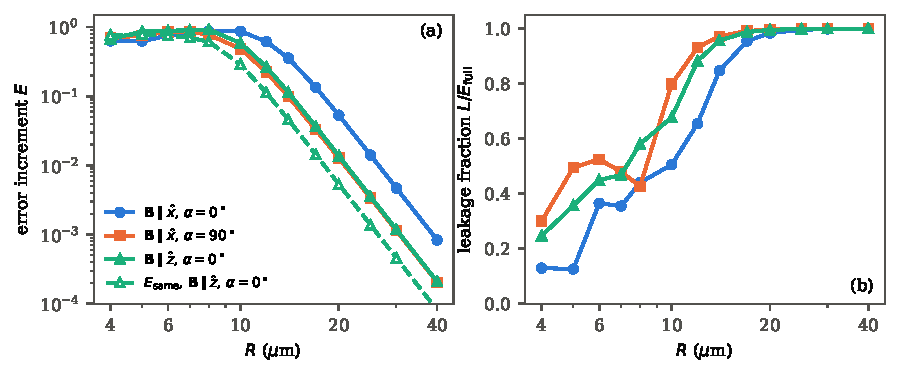
\includegraphics[width=0.85\textwidth]{figures/fig1_error_map.pdf}
\caption{Error increment caused by one $P$-state contaminant in a neighbouring CZ pair, for the gate of Ref.~\cite{Evered2023} ($^{87}$Rb $53S_{1/2}$, $\Omega/2\pi=4.6\MHz$, $B=8.5$~G, $d=2\um$, $450\MHz$ blockade), from the three-atom model of Sec.~\ref{sec:model} with contaminant states weighted by the $300$~K BBR rates into $52P_J$ and $53P_J$. (a) Increment of the entanglement infidelity, leakage included, versus the distance $R$ between the contaminant and the pair centre, for in-plane angle $\alpha$ from the pair axis and bias-field directions as labelled. Solid: contaminant present throughout the gate ($E_{\rm full}$). Dashed, open symbols: contaminant created during the same gate ($E_{\rm same}$), averaged over its creation time with weight $p_r(t)$. Beyond $25\um$ all curves fall as $R^{-6}$ (fitted slopes $-5.97$ to $-6.04$). (b) Fraction of $E_{\rm full}$ that is leakage out of the qubit space.}
\label{fig:map}
\end{figure*}

Figure~\ref{fig:map} shows the error map at $\Omega/2\pi=4.6\MHz$. A contaminant within about $8\um$ of a pair causes an error increment of $0.6$--$0.9$: the gate fails. The half-error radius, where $E_{\rm full}=0.5$, is $10$--$12\um$ depending on the field direction and the angle $\alpha$. With $\bm B$ along the pair axis the map is anisotropic: at $12\um$, $E_{\rm full}=0.62$ along the axis and $0.22$ perpendicular to it, and the error is suppressed near $\alpha\approx60^\circ$, the node of $1-3\cos^2\theta$. With $\bm B$ normal to the plane the in-plane map is nearly isotropic, $E_{\rm full}=0.59$ at $10\um$ and $0.013$ at $20\um$.

Beyond about $20\um$ the error is perturbative. The exchange coupling $V=C_3/R^3$ acts for a time of order $T$, so the transferred amplitude is of order $VT$ and the error of order $(VT)^2\propto R^{-6}$. The fitted slope of $\ln E_{\rm full}$ against $\ln R$ on $25$--$40\um$ is $-5.97$ to $-6.04$ for all field directions and angles, which we had fixed in advance as a check ($-6.0\pm0.3$). Figure~\ref{fig:map}(b) shows that in this regime the error is almost entirely leakage: the fraction is $0.2$--$0.5$ for $R\le8\um$, above $0.9$ for $R\ge14\um$, and $1.00$ for $R\ge20\um$. The long-range mechanism is therefore not a phase error but the hopping of the $P$ excitation onto a gate atom that is in $53S$ during the pulse; the gate atom is left in a Rydberg $P$ state and is subsequently lost.

A contaminant created during the same gate is less harmful at long range, $E_{\rm same}/E_{\rm full}=0.39$ for $R\ge17\um$, because on average it is present for only part of the pulse. At $R\le12\um$ the ratio is $0.5$--$1.3$: a contaminant that appears mid-pulse can leave the pair in a superposition that the remaining pulse does not undo, which is at short range more harmful than a static perturbation present from the start.

%=====================================================================
\section{Array-level excess error and the time between gates}
\label{sec:array}

\subsection{Delay law}

Consider identical layers of parallel CZ gates separated by a time $t\gg T$. Assume (i) contaminants are rare enough that at most one interacts with a given pair at a time, (ii) each atom becomes a contaminant independently with probability $p_c$ per gate, (iii) a contaminant created a time $t'$ earlier harms a gate with probability $S(t')E_{\rm full}(\bm r(t'))$, where $S$ is its survival probability in $n'P$ and $\bm r(t')$ its position relative to the pair, and (iv) contributions from different contaminants add. Here, the sum over sources $i$ runs over the two atoms of every other gate site. The excess error per CZ, averaged over sites, is then
\begin{equation}
\epsilon(t)=p_c\sum_i\Big[E_{\rm same}(\bm r_i)+\sum_{j\ge1}S(jt)\,E_{\rm full}\big(\bm r_i(jt)\big)\Big].
\label{eq:eps}
\end{equation}
For static contaminants with $S(t)=e^{-t/\tau_P}$ the sum over earlier layers is geometric, and
\begin{equation}
\epsilon(t)=p_c\Big[n_{\rm same}+\frac{n_{\rm full}}{e^{t/\tau_P}-1}\Big],
\label{eq:eps_static}
\end{equation}
where $n_{\rm full}=\sum_iE_{\rm full}(\bm r_i)$ and $n_{\rm same}=\sum_iE_{\rm same}(\bm r_i)$ are error-weighted numbers of neighbours. The delay needed to bring the contribution of earlier layers below a budget $\epsilon^*$ is
\begin{equation}
t_{\rm wait}=\tau_P\ln\!\Big(1+\frac{p_cn_{\rm full}}{\epsilon^*-p_cn_{\rm same}}\Big),
\label{eq:twait}
\end{equation}
when the same-layer term is included in the budget, or Eq.~(\ref{eq:twait}) with $n_{\rm same}=0$ when it is not. The term $p_cn_{\rm same}$ does not depend on $t$: no delay removes it, and if $p_cn_{\rm same}\ge\epsilon^*$ no finite $t_{\rm wait}$ exists. Eqs.~(\ref{eq:eps_static}) and (\ref{eq:twait}) were checked by an independent derivation from the stated assumptions alone.

\subsection{Contaminant motion}

The contaminant does not stay at its site. When the tweezers return after the gate, a Rydberg atom sees approximately the ponderomotive potential of a free electron plus the light shift of the ionic core. At $852$~nm, the trap wavelength of Ref.~\cite{Bluvstein2026}, the free-electron polarisability is $\alpha_e=-1/\omega^2=-349.7$ atomic units, the core contributes $9.08$, and the ground-state polarisability is $\alpha_g=2071.5$ (ARC). A contaminant therefore sits on a repulsive hill of height $(349.7-9.1)/2071.5=0.164$ times the ground-state trap depth $U_g$. For $U_g=1$~mK, as reported for Ref.~\cite{Evered2023}, the hill height is $164\,\mu$K$\times k_B$, the asymptotic speed after the atom rolls off is $v_\infty=(2\times0.164\,U_g/m)^{1/2}=0.177\um/\mu$s, and for a $1\um$ waist the displacement near the hilltop $e$-folds in $3.99\us$, so the atom leaves its site within $14$--$16\us$ from the $10\,\mu$K thermal spread. Every other site is a repulsive hill of the same height. Neither the waist nor the depth during the gate-zone benchmarks is given in Ref.~\cite{Bluvstein2026}; we therefore treat $U_g\in\{0.5,1,2\}$~mK and $w\in\{0.8,1.0,1.2\}\um$ as a declared range rather than as sourced values.\footnote{Ref.~\cite{Bluvstein2026} states that trap intensities in the entangling zone are half of those in the readout zones; we have no absolute value. The orbit-averaging correction to the ponderomotive shift for $n'\approx52$ in a $1\um$ waist lowers the hill by $4$--$7\%$ and $v_\infty$ by $2$--$4\%$; it is neglected.}

We integrate classical trajectories (velocity Verlet, $0.05\us$ step) through the full repulsive landscape of a $15\times15$-site patch with two atoms per site, from the thermal distribution of the ground-state trap at $10\,\mu$K, with 200 trajectories per source atom, and evaluate Eq.~(\ref{eq:eps}) with $E_{\rm full}$ interpolated in $\ln R$ and angle. Over $100\us$ a contaminant travels about $18\um$, small compared with the $\approx150\um$ extent of the gate zone. Ejection from the tweezer therefore redistributes contaminants over the array instead of removing them, and in the bulk of a large array the earlier-layer excess is limited by decay, Eq.~(\ref{eq:eps_static}), rather than by motion.

\subsection{Comparison with the measured dependence on the time between gates}

\begin{figure}[t]
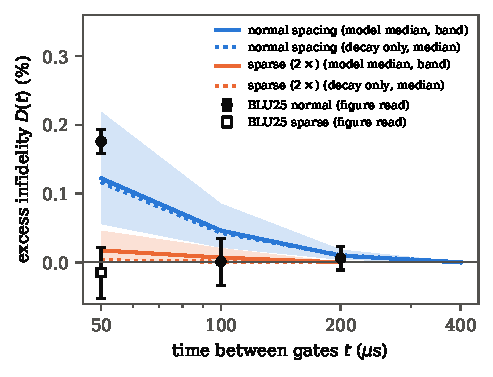
\includegraphics[width=\columnwidth]{figures/fig2_fig6g.pdf}
\caption{Excess CZ infidelity versus the time between gate layers. Symbols: values read from ED Fig.~6g of Ref.~\cite{Bluvstein2026} (RB fidelity, error bars as plotted), expressed as $D(t)=F(400\us)-F(t)$ for normal spacing and $F(200\us)-F(t)$ for the sparse ($2\times$ separation) array, which has no $400\us$ point; the $400\us$ error bar is taken as $0.010\%$. Lines and bands: model, Eq.~(\ref{eq:eps}), with no fitted parameter, at $300$~K and $\Omega/2\pi=4.6\MHz$; bands are the minimum to maximum over the declared input range ($U_g\in\{0.5,1,2\}$~mK, $w\in\{0.8,1.0,1.2\}\um$, pair axis along either lattice direction, $\bm B$ along $x$, $y$ or $z$, assignment of the two lattice pitches, leakage counted or not, fidelity convention factor $f\in\{0.8,1.0\}$). Solid: median with classical contaminant motion; dotted: median for static contaminants (decay only). Geometry: 8 rows $\times$ 16 columns of gate sites, pitch $8.571\um\times12.0\um$ (see text), pair separation $2\um$.}
\label{fig:6g}
\end{figure}

Bluvstein \textit{et al.}\ measured the RB CZ fidelity in a gate zone of 8 rows and 16 columns for times between gates of $50$, $100$, $200$ and $400\us$, and for a sparse array with twice the separation between gate sites \cite{Bluvstein2026}. The data, read from the published figure, are $99.312(15)\%$, $99.487(33)\%$, $99.482(14)\%$ and $99.488\%$ (error bar below about $0.010\%$) for normal spacing, and $99.558(20)\%$, $99.474(25)\%$ and $99.543(31)\%$ at $50$, $100$ and $200\us$ for the sparse array. The site pitch of the benchmark is not stated. We take the row pitch as $60\um/7=8.571\um$, from the statement that the Rydberg beams cover 7 rows over $60\um$ \cite{Bluvstein2026}, and the column pitch as $12.0\um$, read from a figure of the same work.\todo{CONFIRM?: pitch; $60\um/6=10.0\um$ is an equally literal reading of the same sentence} The RB fidelity convention (average-gate versus entanglement fidelity) and the treatment of loss in the RB fit are not stated; we include both as the factor $f\in\{0.8,1.0\}$ and leakage counted or not. Same-layer errors cancel in $D(t)$, which therefore tests only the earlier-layer term of Eq.~(\ref{eq:eps}).

We fixed the comparison in advance: the model fails if, at any of the four points, its band does not overlap the $2\sigma$ interval of the data. Table~\ref{tab:6g} and Fig.~\ref{fig:6g} show that the bands overlap at all four points. The model gives the size of the $50\us$ excess (median $0.122\%$ against $0.176(18)\%$ measured), its disappearance by $100$--$200\us$, and a small or zero effect at twice the spacing. The test has two weaknesses that we state plainly. First, the band spans a factor of four at $50\us$, dominated by the trap depth, the field direction and the fidelity convention, so the agreement is a weak confirmation. Second, a model with static contaminants passes the same test, so the data do not show that motion is required; an inference to the contrary that we made before the calculation is not supported.

\begin{table*}[!tp]
\caption{Pre-registered comparison with ED Fig.~6g of Ref.~\cite{Bluvstein2026}. Data: $D(t)$ in percent with $2\sigma$ interval (figure reading). Model: minimum to maximum over the declared input range of Fig.~\ref{fig:6g}, and median.}
\label{tab:6g}
\begin{ruledtabular}
\begin{tabular}{lccc}
Point & Data $2\sigma$ (\%) & Motion model (\%) & Static model (\%)\\ \hline
Normal, $50\us$ & $[0.140,0.212]$ & $[0.056,0.218]$; $0.122$ & $[0.042,0.247]$\\
Normal, $100\us$ & $[-0.067,0.069]$ & $[0.022,0.085]$; $0.046$ & $[0.016,0.091]$\\
Normal, $200\us$ & $[-0.028,0.040]$ & $[0.004,0.018]$; $0.010$ & $[0.004,0.022]$\\
Sparse, $50\us$ & $[-0.089,0.059]$ & $[0.005,0.046]$; $0.018$ & $[0.000,0.022]$\\
\end{tabular}
\end{ruledtabular}
\end{table*}

A second comparison was made after the data had been seen and is reported as such. At long times between gates the normal and sparse arrays differ only by the same-layer floor $p_cn_{\rm same}$. The model gives this floor as $0.7$--$1.1\times10^{-3}$ for normal spacing and $1.7$--$6.9\times10^{-5}$ for sparse spacing, so the predicted difference, including the factor $f$, is $5.0\times10^{-4}$ to $1.06\times10^{-3}$, plus $0.4$--$1.4\times10^{-4}$ from earlier layers at $200\us$. The measured difference at $200\us$ is $99.543(31)\%-99.482(14)\%=6.1(3.4)\times10^{-4}$.

%=====================================================================
\section{Same-layer floor}
\label{sec:floor}

\subsection{Size and the delay needed for earlier layers}

In the gate-zone geometry above at $300$~K and $4.6\MHz$, the same-layer floor $p_cn_{\rm same}$ is $6.9\times10^{-4}$ to $1.08\times10^{-3}$ per CZ over the declared range (median $1.05\times10^{-3}$). It exceeds $10^{-4}$ for every variant, so a budget of $10^{-4}$ per CZ for the total contaminant error cannot be met by any delay at this density. The contribution of earlier layers alone falls to $10^{-4}$ after $235$--$300\us$ and to $10^{-5}$ after about $500\us$ (Eq.~(\ref{eq:twait}) and the trajectory model agree within the range). These delays are shorter than the $400\us$ between gates used in the QEC circuits of Ref.~\cite{Bluvstein2026} for $10^{-4}$ and comparable to it for $10^{-5}$, consistent with their observation that the effect is absent in those circuits.

\subsection{Dependence on pitch and temperature}

\begin{figure*}[!tp]
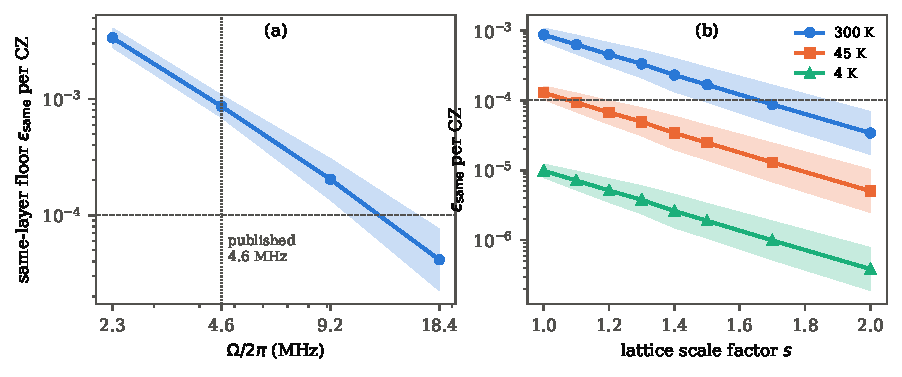
\includegraphics[width=0.85\textwidth]{figures/fig3_floor.pdf}
\caption{Same-layer floor $\epsilon_{\rm same}=p_cn_{\rm same}$ per CZ in the gate-zone geometry of Fig.~\ref{fig:6g}. Bands: minimum to maximum over pair axis, field direction, pitch assignment and trap parameters; lines: geometric mean of the band edges. Dashed line: $10^{-4}$. (a) Versus Rabi frequency at $300$~K, with the pulse shape fixed ($\Omega T/2\pi=1.215$) and $E_{\rm same}$ recomputed at each $\Omega$ on a 6-point creation-time grid (checked against the 12-point grid at $4.6\MHz$ to $2\times10^{-3}$ relative). (b) Versus a common scale factor $s$ applied to both lattice pitches, at $4.6\MHz$, for an ideal Planck field at $300$, $45$ and $4$~K (ARC rates, Table~\ref{tab:T}).}
\label{fig:floor}
\end{figure*}

Because the floor is set by $E_{\rm same}$ at the neighbouring sites, it falls steeply with pitch. Figure~\ref{fig:floor}(b) shows it for both pitches multiplied by a common factor $s$. At $300$~K the floor reaches $10^{-4}$ at $s_{\rm min}=1.5$--$2.0$. Since $E_{\rm same}$ does not depend on temperature, the floor scales with $\Gamma_{\rm BBR}$ alone: for an ideal $45$~K field it is $1.0$--$1.6\times10^{-4}$ at $s=1$ with $s_{\rm min}=1.1$--$1.2$, and at $4$~K it is $0.8$--$1.2\times10^{-5}$. Cooling lengthens $\tau_P$ (Table~\ref{tab:T}), so the delay for the earlier layers does not shrink in proportion: for $10^{-5}$ it rises from about $500\us$ at $300$~K to about $760\us$ at $45$~K, while at $4$~K it is about $300\us$. These cryogenic numbers assume an ideal Planck field. Zhang \textit{et al.}\ measured an effective temperature of $188(8)$~K behind a $45$~K shield \cite{Zhang2026}; at $188$~K the floor is lower than at $300$~K by only a factor of $1.6$ (Table~\ref{tab:T}).

\subsection{Dependence on gate speed}

At fixed pulse shape, $I_r\propto T\propto\Omega^{-1}$, so $p_c\propto\Omega^{-1}$; the computed values $p_c\Omega$ are constant to $0.2\%$ between $2.3$ and $18.4\MHz$. In the perturbative tail $E\propto(VT)^2\propto\Omega^{-2}$ at fixed $R$, and the half-error radius, set by $VT\sim1$, scales as $\Omega^{-1/3}$. Hence the floor should scale as $\Omega^{-3}$ if it is dominated by the tail, and as $\Omega^{-1}\times R_{1/2}^2\propto\Omega^{-5/3}$ if it is dominated by the sites inside $R_{1/2}$ of a two-dimensional array. We recomputed the maps at $\Omega/2\pi=2.3$, $9.2$ and $18.4\MHz$ with the pulse shape fixed. The tail slope is $-5.96$ to $-6.04$ at every $\Omega$, and $E_{\rm full}(30\um)$ falls by $58.7$--$59.2$ between $2.3$ and $18.4\MHz$, against $64$ for exact $\Omega^{-2}$ scaling (both checks fixed in advance). The half-error radius shrinks from $12.8\um$ to $6.8\um$ over this range, a factor $1.88$ against $2.0$ for $\Omega^{-1/3}$.

Figure~\ref{fig:floor}(a) and Table~\ref{tab:floor} give the floor. It is $2.8$--$4.1\times10^{-3}$ at $2.3\MHz$, $0.7$--$1.1\times10^{-3}$ at $4.6\MHz$, $1.4$--$3.1\times10^{-4}$ at $9.2\MHz$ and $2.3$--$7.6\times10^{-5}$ at $18.4\MHz$. The local exponent $d\ln\epsilon_{\rm same}/d\ln\Omega$ moves from $-1.8$ to $-2.0$ at low $\Omega$ to $-2.0$ to $-2.6$ between $9.2$ and $18.4\MHz$, between the two limits above, as the nearest sites leave the half-error radius. Interpolating, the floor reaches $10^{-4}$ at $\Omega/2\pi\approx10$--$16\MHz$ in this geometry at $300$~K. Peak Rabi frequencies of about $2\pi\times17\MHz$ on the same $53S$ state have been used in Ref.~\cite{Evered2026}. This estimate excludes the error channels that change with $\Omega$ and are not in our model, such as intermediate-state scattering, finite blockade and pulse distortion.

\begin{table}[t]
\caption{Same-layer floor per CZ (range over the declared inputs) in the gate-zone geometry, versus Rabi frequency and environment temperature. The $300$~K row is computed; other rows are the $300$~K values scaled by $\Gamma_{\rm BBR}(T)/\Gamma_{\rm BBR}(300\,\mathrm{K})$ from Table~\ref{tab:T}, which is exact within the model because $E_{\rm same}$ does not depend on $T$.}
\label{tab:floor}
\begin{ruledtabular}
\begin{tabular}{lcccc}
$T_{\rm env}$ & $2.3\MHz$ & $4.6\MHz$ & $9.2\MHz$ & $18.4\MHz$\\ \hline
300 K & 2.8--4.1e-3 & 6.9e-4--1.1e-3 & 1.4--3.1e-4 & 2.3--7.6e-5\\
188 K & 1.7--2.5e-3 & 4.3--6.8e-4 & 0.8--1.9e-4 & 1.4--4.8e-5\\
45 K & 4.1--6.0e-4 & 1.0--1.6e-4 & 2.0--4.5e-5 & 3.3--11e-6\\
4 K & 3.1--4.6e-5 & 7.8--12e-6 & 1.5--3.5e-6 & 2.6--8.7e-7\\
\end{tabular}
\end{ruledtabular}
\end{table}


\subsection{Logical consequence of the correlated floor}
\label{sec:logical}

The same-layer floor is spatially correlated: one contaminant makes the nearest gate pairs of the layer fail together. To see whether this matters beyond the marginal rate we simulated a rotated surface-code memory (Z basis, $d$ rounds, $d=3,5,7$) with Stim and PyMatching. Here, every two-qubit layer of the syndrome-extraction circuit is mapped onto gate sites of the lattice of Sec.~\ref{sec:array} (site centres on a grid of $8.571\um\times12.0\um$, two atoms $2\um$ apart per site); each atom becomes a contaminant with probability $mp_c$ per layer ($m=1$ is the physical $300$~K value), and it makes every other pair of the layer fail with probability $E_{\rm same}$ from Fig.~\ref{fig:map}. A failed pair is fully depolarised, which is the effect of an undetected loss. In the correlated model the pairs with $E_{\rm same}\ge0.05$ around one source (the nearest sites, up to four) fail jointly with the exact subset probabilities; in the comparison model every pair fails independently with the same marginal probability. The baseline noise is uniform depolarisation of strength $p$ after every gate, reset and measurement, swept as an unsourced reference. The placement of code qubits in the gate zone of Ref.~\cite{Bluvstein2026} is not published, so this layout is an assumption.

Table~\ref{tab:logical} gives the logical error per round. At the physical strength ($m=1$, $p=10^{-3}$), the excess logical error caused by the correlated contaminant term is $X=6.3$ to $9.8$ times that caused by independent errors with the same per-pair rate, with non-overlapping $95\%$ intervals at every distance; at $p=2\times10^{-3}$ the factor is $3.7$ to $5.6$, and at three or ten times the physical strength it is $2.0$ to $7.7$. At $d=7$ it raises the logical error per round from $9.3\times10^{-7}$ to $2.5\times10^{-5}$, against $4.7\times10^{-6}$ for the independent model. The ratio does not grow from $d=5$ to $d=7$, so in this range the correlation acts as a large prefactor rather than as a loss of effective distance; we had expected the latter. The result is insensitive (about $1\%$) to the internal Pauli structure of a correlated event, to the field direction and to the cluster threshold, and decoding the correlated samples with the independent error model gives the same rates, so a matching decoder does not use the correlation. A heralded-erasure treatment of the loss, a correlation-aware decoder and earlier-layer contaminants were not simulated.

\begin{table*}[!tp]
\caption{Logical error per round of a rotated surface-code memory with $d$ rounds, from Stim and PyMatching, at baseline depolarisation $p=10^{-3}$ and the physical contaminant strength ($m=1$, $p_c=2.53\times10^{-4}$, $300$~K). Brackets: $95\%$ Wilson intervals (every point has at least 100 failures or $10^6$ shots). $X$ is the contaminant excess of the correlated model divided by that of the independent model with equal per-pair marginals.}
\label{tab:logical}
\begin{ruledtabular}
\begin{tabular}{cllll}
$d$ & baseline & correlated & independent & $X$\\ \hline
3 & $1.50\times10^{-4}$ & $7.86\,[7.55,8.18]\times10^{-4}$ & $2.32\,[2.16,2.50]\times10^{-4}$ & $7.8\,[5.2,13.4]$\\
5 & $1.26\times10^{-5}$ & $2.37\,[2.24,2.51]\times10^{-4}$ & $3.56\,[3.07,4.12]\times10^{-5}$ & $9.8\,[6.8,15.3]$\\
7 & $9.3\times10^{-7}$ & $2.47\,[2.13,2.87]\times10^{-5}$ & $4.73\,[4.01,5.59]\times10^{-6}$ & $6.3\,[4.2,9.7]$\\
\end{tabular}
\end{ruledtabular}
\end{table*}

%=====================================================================
\section{Discussion}
\label{sec:discussion}

\textit{What is shown.} Within the model of Sec.~\ref{sec:model}, a single BBR contaminant defeats a gate within $8\um$, has a half-error radius of $10$--$12\um$ at $4.6\MHz$, and beyond $20\um$ causes almost pure leakage with an $R^{-6}$ tail. Combined with the contaminant's survival, this accounts without a fitted parameter for the measured recovery of the CZ fidelity between $50$ and $200\us$ and for the absence of the effect at twice the spacing \cite{Bluvstein2026}. The same model contains a same-layer floor whose size at the benchmark density, $0.7$--$1.1\times10^{-3}$, is consistent with the measured normal-sparse difference at long delays.

\textit{What is model-dependent.} The absolute floor depends on inputs that the experimental papers do not state: the site pitch of the benchmark, the field direction relative to the array and the RB fidelity convention. Our pitch is partly a figure reading. A common scale factor $s=1.2$ on both pitches lowers the floor by a factor of about two [Fig.~\ref{fig:floor}(b)]; the alternative reading of the row pitch noted above changes one pitch only, by $17\%$, and would have a smaller effect, which we have not computed. The trap depth and waist enter only the motion and do not change the decay-limited conclusion for large arrays. Omitted BBR channels (about one third of transfers) and multi-contaminant events make the floor a lower bound in that respect; for the geometry here there are eight atoms (four sites) within the half-error radius of a pair, so the probability of two simultaneous contaminants in that region is of order $(8p_c)^2\approx4\times10^{-6}$, so the single-contaminant approximation holds.

\textit{What is extrapolated.} The temperature dependence assumes an ideal Planck spectrum, which real cryostats do not reach \cite{Zhang2026}. The gate-speed dependence holds the pulse shape, $n$ and the blockade fixed and omits the other errors that grow with $\Omega$. The logical penalty of Sec.~\ref{sec:logical} rests on an assumed placement of code qubits in the gate zone, treats every failure as an undetected loss, and uses a matching decoder; loss detection, which converts part of the error into erasures, and correlation-aware decoding would both reduce it by amounts we have not computed.

The temperature, pitch and speed dependences also bound when the effect sets the cycle time of an error-corrected processor. For the earlier layers, $t_{\rm wait}$ for $10^{-4}$ per CZ is $235$--$300\us$ at $300$~K, below the $400\us$ of Ref.~\cite{Bluvstein2026}. Against the kinematic lower bound of $92\us$ on the in-zone interval derived for the same architecture in Ref.~\todo{REF?: wall-clock model}, the thermal wait is larger by a factor of about three. Over a full QEC round, however, which also contains atom transport and readout, the thermal floor $T_{\rm th}=Lt_{\rm wait}+t_{\rm ro}$ (with $L$ gate layers per round and readout time $t_{\rm ro}$) does not exceed the kinematic floor by the factor of two that would make it the binding constraint: for the surface-code round of Ref.~\cite{Bluvstein2026} the ratio is $0.3$--$2.2$ over our input range, and for transport-dominated lifted-product schedules of Ref.~\todo{REF?: wall-clock model} it is below $1.5$. BBR contaminants therefore constrain the density of a gate layer more than the cycle time.

%=====================================================================
\section{Conclusion}
\label{sec:conclusion}

We have computed, from the published pulse and atomic structure, the error that a blackbody-induced $P$-state contaminant causes in neighbouring Rydberg CZ gates and its consequence in a dense parallel layer. With no fitted parameter the model reproduces the measured recovery of the gate fidelity with the time between gates and with the site separation. Its main new content is a same-layer floor of $0.7$--$1.1\times10^{-3}$ per CZ at current gate-zone density at room temperature, which no delay removes and which falls as $\Omega^{-2}$ to $\Omega^{-2.6}$ with gate speed and in proportion to the BBR rate. The main limitation is that the benchmark geometry and fidelity convention are not published, so the absolute floor carries a factor of about two of input uncertainty. The cleanest test is the CZ infidelity versus gate-site pitch at long inter-gate delay, which the model predicts without parameters; in a surface-code memory the excess logical error from the correlated floor is four to ten times that from independent errors of the same rate, so the next steps are loss detection and correlation-aware decoding in that simulation.

\begin{acknowledgments}
\todo{CONFIRM?: acknowledgments and funding}
\end{acknowledgments}

\bibliography{references}

\end{document}
